%
% 3-liouville.tex
%
% (c) 2026 Prof Dr Andreas Müller
%
\section{Das Prinzip von Liouville
\label{buch:intalg:section:liouville}}
\kopfrechts{Das Prinzip von Liouville}%
Die in Kapitel~\ref{chapter:ratint} durchgerechneten Beispiele 
suggerieren, dass eine Stammfunktion immer nur eine Linearkombination
von Logarithmen der Teilnenner der Partialbruchzerlegung ist.
Das Prinzip von Liouville zeigt, dass dies ganz allgemein gilt.

%
% Das Prinzip
%
\subsection{Das Prinzip 
\label{buch:intalg:liouville:subsection:prinzip}}
Die Erfahrung bei den rationalen Funktionen hat gezeigt, dass die
Stammfunktion immer nur logarithmische Erweiterungen enthält.
Tatsächlich gilt dies ganz allemein, wie der folgende Satz zeigt.

\begin{satz}[Prinzip von Liouville]
Sei $F$ ein Funktionenkörper mit Konstantenkörper $K$ und $f\in F$.
Wenn $f$ eine Stammfunktion $g$ in einer elementaren Erweiterung
$G\supset F$ hat, die den gleichen Konstantenkörper wie $F$ hat, dann
gibt es $v_0,v_1,\dots,v_n\in F$ und $c_1,\dots,c_k\in K$ mit
\begin{equation}
f
=
Dv_0
+
\sum_{i=1}^n c_i\frac{Dv_i}{v_i},
\end{equation}
d.~h.~
\[
\int f(z)\,dz
=
v_0
+ 
\sum_{i=1}^n c_i \log(v_i).
\]
$G$ muss also alle Logarithmen $\log(v_i)$, $i=1,\dots,n$, enthalten.
\end{satz}

Wie kann man überhaupt eine solche Aussage beweisen?
Wenn $g$ die Stammfunktion von $f$ ist, dann muss die Ableitung
von $g$ wieder $f$ ergeben, also $Dg=f$.
Wenn also $g$ in einer Erweiterung $F(\vartheta_1,\dots,\vartheta_n)$
von $F$ liegt, dann kann man versuchen, einen Ausdruck für $g$ in den
Elementen $\vartheta_k$ abzuleiten.
Dabei muss ein Ausdruck entstehen, welcher mit $f$ übereinstimmt.
Alle Terme mit den Elementen $\vartheta_k$ müssen sich daher wegheben.

Der allgemeine Fall einer Erweiterung der Form
$F(\vartheta_1,\dots,\vartheta_n)$ führt zu ziemlich komplizierten
Ausdrücken.
Daher beginnen wir damit einer Erweiterung $F(\vartheta)$ um ein
einziges $\vartheta$.
In diesem Fall muss $g$ die Form einer rationalen Funktion
\begin{equation}
g
=
\frac{a(\vartheta)}{b(\vartheta)} 
=
\frac{
a_0 + a_1\vartheta + \dots a_n\vartheta^n
}{
b_0 + b_1\vartheta + \dots b_m\vartheta^m
}
\label{buch:intalg:liouville:eqn:bruch}
\end{equation}
haben, wobei $a(\vartheta)\in F[\vartheta]$ und
$b(\vartheta)\in F[\vartheta]$ Polynome mit Koeffizienten in $F$ sind.
In diesem Fall lässt sich die Ableitung von $g$ leichter berechnen.
Zu diesem Zweck berechnen wir im
Abschnitt~\ref{buch:intalg:liouville:subsection:polynome}
zunächst die Ableitung von Polynomen von $\vartheta$ für die
verschiedenen Arten von Erweiterungen.
Diese Resultate verwenden wir dann im
Abschnitt~\ref{buch:intalg:liouville:subsection:spezialfaelle},
um das Prinzip von Liouville für eine Erweiterung der Form $F(\vartheta)$
zu beweisen.
In Abschnitt~\ref{buch:intalg:liouville:subsection:allgemein}
wird der allgemeine Fall bewiesen.


%
% Polynome von Erweiterungen
%
\subsection{Polynome von Erweiterungen
\label{buch:intalg:liouville:subsection:polynome}}
Die oben formulierte Beweisstrategie für das Prinzip von Liouville
basiert darauf, dass wir die Ableitung der Stammfunktion ausrechnen
und dann nachweisen, dass nur logarithmische Terme als Ableitung
Ausdrücke in $F$ ergeben.
Dazu müssen zunächst die Ableitungen von Zähler und Nenner in
\eqref{buch:intalg:liouville:eqn:bruch}
verstanden werden, was in den folgenden Abschnitten geklärt werden
soll.

%
% Polynome einer logarithmischen Erweiterung
%
\subsubsection{Polynome einer logarithmischen Erweiterung}
Das Prinzip von Liouville verspricht, dass nur logarithmische Erweiterungen
für die Stammfunktion gebraucht werden, und dass diese nur linear
vorkommen.
Dies wird sich darin äussern, dass die Erweiterung im rationalen Teil
nicht vorkommen kann.
Dies wird sich daraus ergeben, wie genau sich der Grad eines Polynoms
in $\vartheta$ beim Ableiten ändert.
Der folgende Satz gibt darüber Auskunft.

\begin{satz}
\label{buch:intalg:liouville:polynome:satz:logarithmisch}
Sei $F$ ein Funktionenkörper mit Konstantenkörper $K\subset F$ und sei
$\vartheta$ ein logarithmisch transzendentes Element über $F$ mit
$\vartheta=\log u$ mit $u\in F$.
Sei ausserdem
$a(\vartheta) = a_0+a_1\vartheta+\dots+a_n\vartheta^n\in F[\vartheta]$
ein Polynom in $\vartheta$ mit Koeffizienten in $F$.
Dann gilt:
\begin{enumerate}
\item
Die Ableitung von $a(\vartheta)$ ist ebenfalls ein Polynom mit Koeffizienten
in $F$: $Da(\vartheta)\in F[\vartheta]$.
\item
Wenn der Leitkoeffizient $a_n$ eine Konstante ist, dann ist
$\deg Da(\vartheta)=\deg a(\vartheta) -1$.
\item
Wenn der Leitkoeffizient $a_n$ keine Konstante ist, dann ist
$\deg Da(\vartheta)=\deg a(\vartheta)$.
\end{enumerate}
\end{satz}

\begin{proof}
\begin{enumerate}
\item
Die Ableitung ist
\begin{align*}
Da(\vartheta)
&=
D\sum_{k=0}^n a_k\vartheta^k
=
\sum_{k=0}^n \bigl(Da_k\vartheta^k + a_kk\vartheta^{k-1}D\vartheta\bigr)
\\
&=
\sum_{k=0}^n Da_k\vartheta^k
+
D\vartheta \sum_{k=0}^{n-1} a_{k+1}(k+1)\vartheta^k
\\
&=
\sum_{k=0}^{n-1} \bigl(Da_k+(k+1)a_{k+1}D\vartheta\bigr) \vartheta^k
+
Da_n \vartheta^n
\\
&=
\sum_{k=0}^{n-1}
\biggl(
\underbrace{Da_k+(k+1)a_{k+1}\frac{Du}{u}}_{\displaystyle\in F}
\biggr) \vartheta^k
+
Da_n \vartheta^n
\end{align*}
Da $Du\in F$ und $u\in F$ folgt, dass der Koeffizient in der Klammer
ebenfalls in $F$ ist und daher ist $Da(\vartheta)\in F[\vartheta]$.
\item
Wenn $a_n$ eine Konstante ist, dann fällt der Term mit $\vartheta^n$ weg,
der Grad von $Da(\vartheta)$ ist also höchstens $n-1$.
Es ist zu zeigen, dass der Grad genau $n-1$ ist, d.~h.~dass der Koeffizient
von $\vartheta^{n-1}$ nicht verschwindet.
Würde dieser Koeffizient verschwinden, dann wäre wegen $Da_n=0$
\begin{align*}
0
&=
Da_{n-1} + na_n D\vartheta
\\
&=
D(a_{n-1}+na_n\vartheta),
\end{align*}
d.~h.~$a_{n-1}+na_n\vartheta=c$ ist eine Konstante $c\in K$.
Die Gleichung
\[
na_n\cdot\vartheta
+
(\underbrace{a_{n-1}-c}_{\displaystyle\in K})
=
0
\]
bedeutet aber, dass $\vartheta$ algebraisch ist über $K$.
Dies widerspricht der Voraussetzung, dass $\vartheta$ transzendent ist.
Der Widerspruch zeigt, dass $\deg Da(\vartheta)=n-1$ ist.
\item
Wenn $a_n$ keine Konstante ist, dann ist $Da_n\ne 0$ und damit
$\deg Da(\vartheta)=n$.
\qedhere
\end{enumerate}
\end{proof}

%
% Polynome einer exponentiellen Erweiterung
%
\subsubsection{Polynome einer exponentiellen Erweiterung}
Im Gegensatz zu einer logarithmischen Erweiterung nimmt der Grad
eines Polynoms einer exponentiellen Erweiterung beim Ableiten nicht ab.

\begin{satz}
\label{buch:intalg:liouville:polynome:satz:exponentiell}
Sei $F$ ein Funktionenkörper mit Konstantenkörper $K\subset F$ und sei
$\vartheta$ ein exponentielles transzendentes Element über $F$ mit
$\vartheta=\exp u$ mit $u\in F$.
Sei ausserdem
$a(\vartheta) = a_0+a_1\vartheta+\dots+a_n\vartheta^n\in F[\vartheta]$
ein Polynom in $\vartheta$ mit Koeffizienten in $F$.
Dann gilt:
\begin{enumerate}
\item
Für $h\in F$ und $n\ne 0$ gilt $D(h\vartheta^n) = \bar{h}\vartheta^n$ mit
$\bar{h}\in F$ und $\bar{h}\ne 0$.
\item
Für ein Polynom
$a(\vartheta)\in F[\vartheta]$
gilt
$\deg Da(\vartheta) = \deg a(\vartheta)$.
\item
$a(\vartheta) \in F[\vartheta]$
teilt $Da(\vartheta)$ genau dann, wenn $a(\vartheta)$ ein Monom ist,
also $a(\vartheta)=h\vartheta^n$ mit $h\in F\setminus\{0\}$, $n\in\mathbb{Z}$.
\end{enumerate}
\end{satz}

\begin{proof}
\begin{enumerate}
\item
Die Ableitung ist
\[
D(h\vartheta^n)
=
Dh\cdot\vartheta^n + hn\vartheta^{n-1}D\vartheta
=
Dh\cdot\vartheta^n + hn\vartheta^{n-1} \vartheta Du
=
(\underbrace{Dh+ hn Du}_{\displaystyle=\bar{h}}) \vartheta^n
\]
Wäre $\bar{h}=0$, dann wäre $h\vartheta^n$ eine Konstante $c\in K$,
d.~h.~es gälte eine Gleichung der Form
\[
h\cdot \vartheta^n - c = 0.
\]
Dies bedeutet, dass $\vartheta$ algebraisch ist über $F$, im Widerspruch
zur Voraussetzung, dass $\vartheta$ transzendent ist.
Somit folgt $\bar{h}\ne 0$.
\item
Die Ableitung des Terms $a_n\vartheta^n$ des Polynoms ist
$\bar{a}_n\vartheta^n$ mit $\bar{a}_n\ne 0$.
Somit ist $\deg Da(\vartheta) = n = \deg a(\vartheta)$.
\item
Wenn $a(\vartheta)$ das Monom $h\vartheta^n$ ist, dann ist
\[
Da(\vartheta)
=
\bar{h}\vartheta^n
=
\frac{\bar{h}}{h}
\cdot
h\vartheta^n
=
\frac{\bar{h}}{h}
\cdot
a(\vartheta),
\]
d.~h.~wegen $\bar{h}/h\in F$ ist $Da(\vartheta)$ ist ein Teiler von
$a(\vartheta)$.

Sei jetzt umgekehrt $Da(\vartheta)$ ein Teiler von $a(\vartheta)$.
Es gibt dann ein $g\in F$ mit $Da(\vartheta)=ga(\vartheta)$.
Sei $m$ der höchste Exponent $<n$ von $\vartheta$ im Polynom $a(\vartheta)$,
welcher einen nicht verschwindenen Koeffizienten $a_m\ne 0$ hat.
Das Polynom hat also die Form
\begin{align*}
a(\vartheta)
&=
a_n\vartheta^n + a_m\vartheta^m + \ldots + a_1\vartheta + a_0
\intertext{mit der Ableitung}
Da(\vartheta)
&=
\bar{a}_n\vartheta^n
+
\bar{a}_m\vartheta^m
+
\ldots
+
\bar{a}_1\vartheta
+
Da_0.
\end{align*}
mit $\bar{a}_k=Da_k+ka_kDu$.
Die Teilbarkeitsbedingung bedeutet dann
\[
\renewcommand{\arraycolsep}{2pt}
Da(\vartheta)
=
ga(\vartheta)
\quad
\Rightarrow
\quad
\left\{\;
\begin{array}{lclclcl}
ga_n &=& \bar{a}_n &=& Da_n &+& na_n Du \\
ga_m &=& \bar{a}_m &=& Da_m &+& ma_m Du.
\end{array}
\right.
\]
Auflösen nach $g$ ergibt
\begin{align*}
g
&=
\frac{Da_n}{a_n} + n\,Du
=
\frac{Da_m}{a_m} + m\,Du.
\intertext{Die Differenz der rechten Seiten ist}
0
&=
\frac{Da_n}{a_n}
-
\frac{Da_m}{a_m}
+
(n-m)\,Du.
%\intertext{Die rechte Seite kann man auch als}
%0
%&=
%D
%\biggl(
%\frac{a_n}{a_m}
%+
%(n-m)u
%\biggr)
\end{align*}
Die rechte Seite ermöglicht auch, die Ableitung
\begin{align*}
D
\biggl(
\frac{a_n}{a_m}\vartheta^{n-m}
\biggr)
&=
\frac{(Da_n) a_m - a_n\,Da_m}{a_m^2} \vartheta^{n-m}
+
(n-m)\vartheta^{n-m}Du
\\
&=
\frac{a_n}{a_m}
\biggl(
\frac{Da_n}{a_n}
-
\frac{Da_m}{a_m}
-
(n-m)Du
\biggr)
=
0
\end{align*}
zu berechnen.
Somit ist $(a_n/a_m)\vartheta^{n-m}$ eine Konstante, was nur für $n-m=0$
möglich ist.
Es gibt also gar keinen Koeffizienten $a_m\ne 0$ mit $m<n$.
Somit ist $a(\vartheta)=a_n\vartheta^n$ ein Monom.
\qedhere
\end{enumerate}
\end{proof}

%
% Polynome einer algebraischen Erweiterung
%
\subsubsection{Polynome einer algebraischen Erweiterung}
Logarithmische und exponentielle transzendente Erweiterungen
sind durch ihre Eigenschaften unter Differentiation charakterisiert.
Damit ist bereits sichergestellt, dass die Ableitung im erweiterten
Funktionenkörper liegt.
Für eine algebraische Erweiterung $F(\vartheta)$ von $F$ ist dies
jedoch nicht selbstverständlich.
Der folgende Satz zeigt, dass auch für eine algebraische Erweiterung
um das algebraische Element $\vartheta$ die Ableitung $D\vartheta$
in $F(\vartheta)$ liegt.

\begin{satz}
\label{buch:intalg:liouville:polynome:satz:algebraisch}
Sei $\vartheta$ ein algebraisches Element über $F$ mit Minimalpolynom
\begin{equation}
0
=
m(\vartheta)
=
m_0 + m_1\vartheta + \ldots + m_{n-1}\vartheta^{n-1} + \vartheta^n
=
\sum_{k=0}^n m_k\vartheta^k
\label{buch:intalg:liouville:polynome:eqn:minimal}
\end{equation}
mit $m_n=1$.
\begin{enumerate}
\item
Die Ableitung von $\vartheta$ hat die Form
\[
D\vartheta
=
-
\frac{d(\vartheta)}{e(\vartheta}
\in
F(\vartheta)
\]
mit Polynomen 
\begin{equation}
d(\vartheta)
=
\sum_{k=0}^{n-1} (Dm_k) \vartheta^k
\qquad\text{und}\qquad
e(\vartheta)
=
\sum_{k=0}^{n-1} (k+1)m_{k+1} \vartheta^k
=
m'(\vartheta).
\label{buch:intalg:liouville:polynome:eqn:zaehlernenner}
\end{equation}
\item
Eine rationale Funktion von $\vartheta$ mit Koeffizienten in $F$
kann immer als Polynom vom Grad höchstens $n-1$ in $\vartheta$
mit Koeffizienten in $F$ geschrieben werden.
\end{enumerate}
\end{satz}

\begin{proof}
\begin{enumerate}
\item
Ableiten von
\eqref{buch:intalg:liouville:polynome:eqn:minimal}
liefert
\begin{align*}
0
=
Dp(\vartheta)
&=
\sum_{k=0}^n (Dm_k)\vartheta^k
+
\biggl(\sum_{k=0}^n km_k\vartheta^{k-1} \biggl)D\vartheta
\\
&=
\sum_{k=0}^{n-1} (Dm_k)\vartheta^k
+
\biggl(\sum_{k=0}^{n-1} (k+1)m_{k+1}\vartheta^k \biggl)D\vartheta
,
\end{align*}
wobei wir $Dm_n=0$ bereits ausgenützt haben.
Auflösen nach $D\vartheta$ liefert
\[
D\vartheta
=
-\frac{
\displaystyle
\sum_{k=0}^{n-1} (Dm_k) \vartheta^k
}{
\displaystyle
\sum_{k=0}^{n-1} (k+1)m_{k+1} \vartheta^k
}
\in
F(\vartheta).
\]
Zähler und Nenner sind die Polynome in
\eqref{buch:intalg:liouville:polynome:eqn:zaehlernenner}
\item
Sei 
\begin{equation}
f(\vartheta)
=
\frac{u(\vartheta)}{v(\vartheta)}
\label{buch:intalg:liouville:polyalg:eqn:bruch}
\end{equation}
ein Quotient von Polynomen mit Koeffizienten in $F$.
Nach Reduktion mit dem Minimalpolynom darf man annehmen, dass
der Grad von Zähler und Nenner kleiner als $n$ ist.
Insbesondere sind $v(Z)$ und das Minimalpolynom $m(Z)$
teilerfremd.
Nach dem erweiterten euklidischen Algorithmus gibt es
Polynome $s(Z)$ und $t(Z)$ mit 
\[
s(Z)v(Z) + t(Z)m(Z) = 1.
\]
Einsetzen von $\vartheta$ bringt den Term mit $m(\vartheta)=0$ zum
verschwinden und liefert
\[
s(\vartheta)v(\vartheta) = 1
\qquad\Rightarrow\qquad s(\vartheta) = \frac{1}{v(\vartheta)}.
\]
Damit ist das inverse Element von $v(\vartheta)$ als Polynom in
$\vartheta$ ausgedrückt.
Für den Bruch~\eqref{buch:intalg:liouville:polyalg:eqn:bruch}
folgt daher
\[
f(\vartheta)
=
\frac{u(\vartheta)}{v(\vartheta)}
=
u(\vartheta)\cdot s(\vartheta).
\]
Die rechte Seite ist ein Polynom.
Mit dem Minimalpolynom kann es weiter auf ein Polynom vom 
Grad $<n$ reduziert werden.
\qedhere
\end{enumerate}
\end{proof}

%
% Beweis des Prinzips von Liouville in Spezialfällen
%
\subsection{Beweis des Prinzips von Liouville in Spezialfällen
\label{buch:intalg:liouville:subsection:spezialfaelle}}
Das Prinzip von Liouville geht davon aus, dass eine Funktion $f$
in einem Funktionenkörper eine Stammfunktion $g$ in einer geeigneten
Erweiterung hat.
Es zeigt dann, dass diese Erweiterung nur Logarithmen von Elementen
in $F$ braucht und dass diese Logarithmen in der Stammfunktion nur 
linear vorkommen.
Beim Ableiten müssen die Terme, die Elemente der Erweiterung enthalten,
wieder verschwinden.
Man muss also für exponentielle und algebraische Erweiterungen zeigen,
dass diese beim Ableiten nicht verschwinden können.
Und für logarithmische Erweiterungen muss man zeigen, dass diese genau
dann verschwinden können, wenn sie linear in der Stammfunktion auftreten.

In diesem Abschnitt beweisen wir dies für eine Erweiterung, die von einem
einzigen zusätzlichen Element erzeugt wird.
Dies ist zwar nicht ausreichend für das Integral
\[
\int \frac{dx}{x^2+1}
=
\frac{1}{2i}\log(x+i)
-
\frac{1}{2i}\log(x-i)
=
\arctan x,
\]
welches zwei unabhängige logarithmische Erweiterungen braucht, aber
die Methode, die wir dabei kennenlernen werden, wird in
Abschnitt~\ref{buch:intalg:liouville:subsection:allgemein}
verallgemeinert, so dass sie auch für kompliziertere Integrale
gilt und damit das liouvillesche Prinzip bestätigt.

%
% Ein Ausdruck für die Stammfunktion
%
\subsubsection{Ein Ausdruck für die Stammfunktion}
In diesem Abschnitt ist $F$ ein Funktionenkörper mit Konstantenkörper
$K$ und $f\in F$ eine Funktion.
Es wird angenommen, dass es eine Stammfunktion $g$ von $f$ in einem
Erweiterungskörper $F(\vartheta)$ gibt.
$g\in F(\vartheta)$ bedeutet aber, dass $g$ ein rationaler Ausdruck
in $\vartheta$ ist.
Insbesondere kann $g$ als
\begin{equation}
g
=
a_0(\vartheta)
+
\frac{a(\vartheta)}{b(\vartheta)}
\label{buch:intalg:liouville:spezial:eqn:bruch}
\end{equation}
geschrieben werden, wobei $a_0(\vartheta)$, $a(\vartheta)$ und $b(\vartheta)$
Polynome mit Koeffizienten in $F$ sind.
Ausserdem darf angenommen werden, dass $a(\vartheta)$ und $b(\vartheta)$
teilerfremd sind, dass also der Bruch in
\eqref{buch:intalg:liouville:spezial:eqn:bruch}
vollständig gekürzt ist und dass
$\deg a(\vartheta)<\deg b(\vartheta)$ gilt.

Wir nehmen ausserdem an, dass $F$ und $F(\vartheta)$ den gleichen
Konstantenkörper haben.
Dies kann immer erreicht werden, indem man alle für das Integral
nötigen Konstanten bereits dem Körper $F$ hinzufügt, bevor man beginnt,
um nichtkonstante Funktionen zu erweitern.

Wir müssen zeigen, dass $\vartheta$ nur ein Logarithmus sein kann und dass
$\vartheta$ nur linear in $g$ vorkommen kann.

%
% Der Fall einer logarithmischen Erweiterung
%
\subsubsection{Der Fall einer logarithmischen Erweiterung}
Das Prinzip von Liouville besagt nicht nur, dass in der Stammfunktion nur
logarithmische Erweiterungen vorkommt, sondern dass sie sogar nur
linear mit konstanten Koeffizienten vorkommen.
In diesem Abschnitt betrachten wir eine einzelne logarithmische
Erweiterungen $F(\vartheta)\supset F$.
Das Prinzip von Liouville besagt in diesem Spezialfall, dass die
Stammfunktion von $f\in F$, falls sie in $F(\vartheta)$ liegt,
die Form $c_0+c_1\vartheta$ haben muss, wobei $c_1$ eine Konstante ist.

\begin{satz}
\label{buch:intalg:liouville:satz:logsimple}
Sei $F(\vartheta)$ eine logarithmische Erweiterung eines Funktionenkörpers
$F$.
$F$ und $F(\vartheta)$ haben den gleichen Konstantenkörper.
Weiter sei $f\in F$ und $g \in F(\vartheta)$ eine Stammfunktion.
Dann ist $g=c_0+c_1\vartheta$ mit $c_0\in F$ und $c_1\in K$.
\end{satz}

\begin{proof}
Der Nenner $b(\vartheta)$ des Ausdrucks 
\eqref{buch:intalg:liouville:spezial:eqn:bruch}
für $g$ kann in die irreduziblen Faktoren
$b_1(\vartheta),\ldots,b_m(\vartheta)$
zerlegt werden.
Weiter dürfen wir annehmen, dass die Faktoren $b_k(\vartheta)$
normierte Polynome sind.
Die zugehörige Partialbruchzerlegung hat daher die Form
\begin{align}
g
&=
a_0(\vartheta)
+
\sum_{k=1}^m
\sum_{i=1}^{r_k}
\frac{a_{ik}(\vartheta)}{b_k(\vartheta)^i},
\label{buch:intalg:liouville:speziell:eqn:f}
\intertext{wobei $a_{ik}(\vartheta)\in F(\vartheta)$ Polynome mit
$\deg a_{ik}(\vartheta) < \deg b_k(\vartheta)$ sind.
Die Ableitung von $g$ ist}
f
=
Dg
&=
Da_0(\vartheta)
+
\sum_{k=1}^m
\sum_{i=1}^{r_k}
D
\frac{a_{ik}(\vartheta)}{b_k(\vartheta)^i}.
\label{buch:intalg:liouville:speziell:eqn:fabgeleitet}
\intertext{Dabei ist wichtig, dass $f\in F$ ist und daher die Erweiterung
$\vartheta$ nicht enthält.
Wir wollen zeigen, dass diese zur Folge hat, dass gar keine Bruchterme
vorkommen können.
Die Ableitung eines einzelnen Terms in der Summe ist}
D
\frac{a_{ik}(\vartheta)}{b_k(\vartheta)^i}
&=
\frac{
Da_{ik}(\vartheta)\cdot b_k(\vartheta)^i
-
a_{ik}(\vartheta)ib_k(\vartheta)^{i-1} Db_k(\vartheta)
}{
b_k(\vartheta)^{2i}
}
\notag
\\
&=
\frac{Da_{ik}(\vartheta)}{b_k(\vartheta)^i}
-
i
\frac{
a_{ik}(\vartheta) Db_k(\vartheta)
}{
b_k(\vartheta)^{i+1}
}.
\label{buch:intalg:liouville:speziell:eqn:abgeleitet}
\end{align}
Die Ableitung $Db_k(\vartheta)$ hat Grad
$\deg Db_k(\vartheta) = \deg b_k(\vartheta)-1$.
Da $b_k(\vartheta)$ irreduzibel ist, sind $Db_k(\vartheta)$
und $b_k(\vartheta)$ teilerfremd.
Die Terme 
\eqref{buch:intalg:liouville:speziell:eqn:abgeleitet}
sind alle vollständig gekürzt.
Die höchste Nennerpotenz von $b_k(\vartheta)$ in
\eqref{buch:intalg:liouville:speziell:eqn:fabgeleitet}
hat den Exponenten $r_k+1$, und sie kommt nur genau einmal
im letzten Summanden vor.
Daher gibt es keinen weiteren Term, mit dem er sich wegheben könnte.
Die Summe in~\eqref{buch:intalg:liouville:speziell:eqn:fabgeleitet}
muss daher verschwinden und $g$ ist nur ein Polynom von $a_0(\vartheta)$.

Da $f=Dg=Da_0(\vartheta)$ nicht von $\vartheta$ abhängen darf, muss
$a_0(\vartheta)$ ein Polynom vom Grad höchstens $1$ sein, also
\[
g
=
a_0(\vartheta) = c_0+c_1\vartheta
\qquad\text{mit $c_k\in F$.}
\]
Damit $\vartheta$ in $Dg$ nicht vorkommt, muss der Grad von des Polynoms
$a_0(\vartheta)$ beim Differenzieren um eins abnehmen, was nur möglich ist,
wenn der Koeffizient von $\vartheta$ eine Konstante ist, also $c_1\in K$.
Somit 
\end{proof}

%
% Der Fall einer exponentiellen Erweiterung
%
\subsubsection{Der Fall einer exponentiellen Erweiterung}
Nach dem Prinzip von Liouville treten in einer Stammfunktion nur
logarithmische Erweiterungen auf.
Eine exponentielle Erweiterung $F(\vartheta)$ sollte also in der
Stammfunktion einer Funktion $f\in F$ gar nicht vorkommen.
Dies zeigt auch der folgende Satz.

\begin{satz}
\label{buch:intalg:liouville:satz:expsimple}
Sei $F(\vartheta)$ eine exponentielle transzendente Erweiterung eines
Funktionenkörpers $F$.
$F$ und $F(\vartheta)$ haben den gleichen Konstantenkörper.
Weiter sei $f\in F$ und $g\in F(\vartheta)$ eine Stammfunktion von $f$.
Dann ist $g\in F$.
\end{satz}

\begin{proof}
Sei also $\vartheta = \exp(u)$ eine Exponentialfunktion von $u\in F$.
Die Stammfunktion $g\in F(\vartheta)$ kann wieder mit einer Zerlegung
in irreduzible Faktoren des Nenners in der Form einer Partialbruchzerlegung
\eqref{buch:intalg:liouville:speziell:eqn:f}
geschrieben werden.

Im Fall einer logarithmischen Erweiterung
(Beweis von Satz~\ref{buch:intalg:liouville:satz:logsimple})
haben wir dann unter Verwendung von
Satz~\ref{buch:intalg:liouville:polynome:satz:logarithmisch}
gezeigt, dass der Term mit der höchsten Nennerpotenz $b_k(\vartheta)^{r_k+1}$
sich gegen nichts wegheben kann.
Dies hat dann gezeigt, dass die Bruchterme in der Stammfunktion nicht
vorkommen können.

Im vorliegenden Fall ist $b_k(\vartheta)$ kein Monom, also nicht von
der Form $h\vartheta^m$.
Nach Aussage 3 von Satz~\ref{buch:intalg:liouville:polynome:satz:exponentiell}
sind also $b_k(\vartheta)$ und $b_k(\vartheta)'$ teilerfremd und damit
die Bruchterme in \eqref{buch:intalg:liouville:speziell:eqn:f}
vollständig gekürzt.
Wie im Fall einer logarithmischen Erweiterung folgt jetzt, dass sich
die Bruchterme nicht wegheben können.
Da auf der linken Seite von \eqref{buch:intalg:liouville:speziell:eqn:f}
$\vartheta$ nicht vorkommen darf, dürfen in der Stammfunktion keine 
Bruchterme vorkommen.

Es bleibt also nur noch der polynomielle Teil.
Nach Satz~\ref{buch:intalg:liouville:polynome:satz:exponentiell}
kann aber der Grad des Polynoms $a_0(\vartheta)$ beim Differenzieren
nicht abnehen, die Ableitung $Da_0(\vartheta)$ kann daher $\vartheta$
nicht enhalten, wenn $a_0(\vartheta)$ ein Polynom vom, Grad 0 ist,
also $g=a_0(\vartheta)=a_{0,0}\in F$.
\end{proof}

%
% Der Fall einer algebraischen Erweiterung
%
\subsubsection{Der Fall einer algebraischen Erweiterung}
Auch für eine algebraische Erweiterung besagt das Prinzip von Liouville,
dass die Stammfunktion einer Funktion des Funktionenkörpers die
Erweiterung gar nicht enthält.

\begin{satz}
\label{buch:intalg:liouville:satz:algsimple}
Sei $F(\vartheta)$ eine algebraische Erweiterung eines
Funktionenkörpers $F$ mit Minimalpolynom $m(X)\in F[X]$.
$F$ und $F(\vartheta)$ haben den gleichen Konstantenkörper.
Weiter sei $f\in F$ und $g\in F(\vartheta)$ eine Stammfunktion von $f$.
Dann ist $g\in F$.
\end{satz}

\begin{proof}
Sei jetzt $\vartheta$ ein algebraisches Element über $F$ mit Minimalpolynom
$p$ mit Koeffizienten in $F$.
Wie früher ist die Stammfunktion $g$ eine rationale Funktion 
in $\vartheta$ mit Koeffizienten in $F$.
Nach Satz~\ref{buch:intalg:liouville:polynome:satz:algebraisch}
lässt sie sich aber auch als Polynom in $\vartheta$ mit Koeffizienten
in $F$ schreiben, wir schreiben $g=a(\vartheta)$ mit $u(Z)\in F[Z]$.
Die Ableitung ist
\[
f
=
Dg
=
Da(\vartheta).
\]
Die Ableitung des Polynoms $a$ in $\vartheta$ mit Koeffizienten
in $F$ ist
\begin{align*}
Da(\vartheta)
&=
\sum_{k=0}^m Da_k\vartheta^k
+
\sum_{k=1}^m ka_k\vartheta^{k-1} D\vartheta
\\
&=
\sum_{k=0}^{m-1}
\bigl(
Da_k
+
(k+1)a_{k+1}
D\vartheta
\bigr)
\vartheta^k
+
Da_m\vartheta^m.
\end{align*}
Darin ist $D\vartheta$ die Ableitung von $\vartheta$, die nach
Satz~\ref{buch:intalg:liouville:polynome:satz:algebraisch}
eine rationale Funktion von $\vartheta$ mit Koeffzienten in $F$ ist.
Es folgt, dass $Dg$ eine rationale Funktion von $\vartheta$ mit
Koeffizienten in $F$ ist, die ihrerseits wieder als Polynom
geschrieben werden kann.

Es muss jetzt noch gezeigt werden, dass aus $f=Dg$ folgt,
dass $a(\vartheta)$ nicht von $\vartheta$ abhängt.
$\vartheta$ ist nicht die einzige Lösung von $m(\vartheta)=0$, wir schreiben
$\vartheta=\vartheta_1$ und $\vartheta_2,\dots,\vartheta_l$ für die
$l=\deg m$ weiteren Lösungen der Gleichung.
Es gilt also
\begin{align}
f
&=
Da(\vartheta_k),\qquad k=1,\dots,l.
\notag
\intertext{Die Summe all dieser Gleichungen ist}
m\cdot f
&=
\sum_{k=1}^l Da(\vartheta_k).
\notag
\intertext{Es folgt}
f
&=
\frac{1}{l}
\sum_{k=1}^l Da(\vartheta_k)
=
Dh
\qquad\text{mit } h=\frac{1}{l} \sum_{k=1}^l a(\vartheta_k)
\label{buch:intalg:liouville:alg:eqn:symmetrisch}
\end{align}
$h$ ist eine symmetrische Funktion in
$\vartheta_1,\dots,\vartheta_l$, nach dem Hauptsatz über symmetrische
Funktionen lassen sich die Koeffizienten von $h$ nach dem Fundamentalsatz
\ref{buch:komplex:fundamental:satz:fundamentalpolynom} über symmetrische
Polynome durch die elementarsymmetrischen Funktionen von
$\vartheta_1,\dots,\vartheta_l$ ausdrücken.
Diese sind jedoch Koeffzienten des Minimalpolynoms $m(X)$ von $\vartheta$,
die alle in $F$ liegen.
Somit hängt die rechte Seite von
\eqref{buch:intalg:liouville:alg:eqn:symmetrisch}
nicht von $\vartheta$ ab.
\end{proof}

%
% Beweis im allgemeinen Fall
%
\subsection{Beweis im allgemeinen Fall
\label{buch:intalg:liouville:subsection:allgemein}}
Der allgemeine Fall handelt von mehr als nur einer Erweiterung.
Gegeben ist wieder ein Funktionenkörper $F$ mit einer Derivation und
$f\in F$.
Der Konstantenkörper von $F$ wird wieder mit $K$ bezeichnet.
Um eine elementare Stammfunktion $g$ zu konstruieren, müssen mehrere
Funktionen $\vartheta_1,\dots,\vartheta_N$ hinzugefügt werden.
Dies geschieht mit einer Kette
\begin{equation}
\begin{tikzcd}[column sep=0pt]
f \arrow[d,tail] &
	& &
	& &
	& &
	& &
	& g \arrow[d,tail]
\\
F & \subset
	& F(\vartheta_1) \arrow[d,equal] & \subset
	& F(\vartheta_1,\vartheta_2) \arrow[d,equal] & \subset
	& \dots & \subset
	& F(\vartheta_1,\dots,\vartheta_{N-1}) \arrow[d,equal] & \subset
	& F(\vartheta_1,\dots,\vartheta_N) \arrow[d,equal]
\\
  &
	& F_1 & \subset 
	& F_2 & \subset 
	& \dots & \subset
	& F_{N-1} & \subset 
	& F_N
\end{tikzcd}
\label{buch:intalg:liouvill:allg:eqn:cd}
\end{equation}
von Körpererweiterungen.
Das Prinzip von Liouville besagt dann, dass $g$ allein in der Form
\begin{align*}
g
&=
v_0 + \sum_i c_i\log v_i
\intertext{mit Ableitung}
f
&=
Dv_0 + \sum_i c_i\frac{Dv_i}{v_i}
\end{align*}
mit $v_i\in F$ und $c_i\in K$.
Die Form von $g$ in $F_N$ ist also sehr speziell.

Die in
Abschnitt~\ref{buch:intalg:liouville:subsection:spezialfaelle}
bewiesenen Spezialfälle besagen, dass im Fall einer einzigen
Körpererweiterung $F\subset F_1$ eine Funktion $f$ mit Stammfunktion
$g\in F_1$ in der Form
\[
f = Dv_0 + c_1 \frac{Dv_1}{v_1}
\qquad\text{oder}\qquad
g = v_0 + c_1\log v_1
\]
geschrieben werden kann.

\begin{definition}[Liouville-Form]
Ist $g\in G$ eine Stammfunktion von $f\in F$, dann heisst
\[
g = v_0 + \sum_i c_i\log v_i \quad \text{mit } v_k \in F, c_i \in K
\]
eine \emph{Liouville-Form} von $g$ bezüglich $F\subset G$.
\end{definition}

Die Spezialfälle von
Abschnitt~\ref{buch:intalg:liouville:subsection:spezialfaelle}
besagen also, dass die Stammfunktion $g$ einer Funktion $f\in F$ nur
dann in $F(\vartheta)$ sein kann, wenn $g$ eine Liouville-Form
bezüglich $F\subset F(\vartheta)$ hat.
Wir können dies durch das Mengendiagramm
\begin{center}
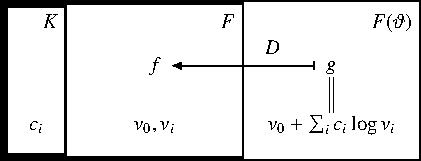
\includegraphics{chapters/070-intalg/images/lf0.pdf}
\end{center}
visualisieren.

Die Spezialfälle von 
Abschnitt~\ref{buch:intalg:liouville:subsection:spezialfaelle}
lassen sich auch auf die Erweiterung
$F_{N-1}\subset F_N = F_{N-1}(\vartheta_N)$ anwenden, die sich
als
\begin{center}
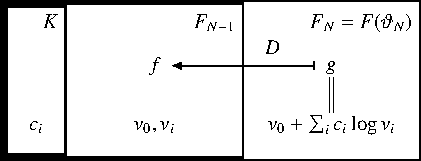
\includegraphics{chapters/070-intalg/images/lfN.pdf}
\end{center}
visualisieren lassen.

Was wir aber erreichen möchten, ist in Abbildung
%
% lf.tex
%
% (c) 2026 Prof Dr Andreas Müller
%
\begin{figure}
\centering
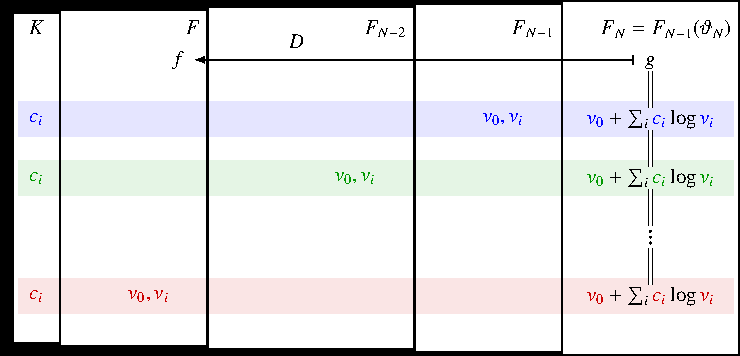
\includegraphics{chapters/070-intalg/images/lf.pdf}
\caption{Allgemeiner Fall des Prinzips von Liouville.
Die Stammfunktion $g\in F_N$ lässt sich in Liouville-Form
bezüglich $F_{N-1}\subset F_N$ mit den blauen Elementen
${\color{blue}c_i}\in K$ und
${\color{blue}v_0}, {\color{blue}v_i}\in F_{N-1}$
schreiben.
Sie muss schrittweise durch neue Elemente in anderen Farben 
in Liouville-Form bezüglich Erweiterungen $F_{k-1}\subset F_k$
umgeschrieben werden, bis die endgültige Liouville-Form mit
roten Elementen ${\color{darkred}c_i}\in K$ und
${\color{darkred}v_0}, {\color{darkred}v_i}\in F$ entsteht.
Dies beweist das Prinzip von Liouville.
\label{buch:intalg:liouville:fig:lf}}
\end{figure}
%
\ref{buch:intalg:liouville:fig:lf} dargestellt.
Zunächst gibt es blaue Elemente
${\color{blue}c_i}\in K$ und
${\color{blue}v_0},{\color{blue}v_i}\in F_{N-1}$, die eine
Liouville-Form für $g$ ergeben.
Diese muss jetzt zunächst in eine Liouville-Form mit den grünen
Elementen
${\color{darkgreen}c_i}\in K$ und
${\color{darkgreen}v_0},{\color{darkgreen}v_i}\in F_{N-2}$ 
bezüglich $F_{N-2}\subset F$ umgewandelt werden.
Durch Wiederholung dieses Prozesses kann man die roten Elemente
${\color{darkred}c_i}\in K$ und
${\color{darkred}v_0},{\color{darkred}v_i}\in F_{N-2}$ 
einer Liouville-Form von $g$ bezüglich $F\subset F_N$ bekommen,
was das Prinzip von Liouville beweist.























